\begin{figure}[tbp]
\centering
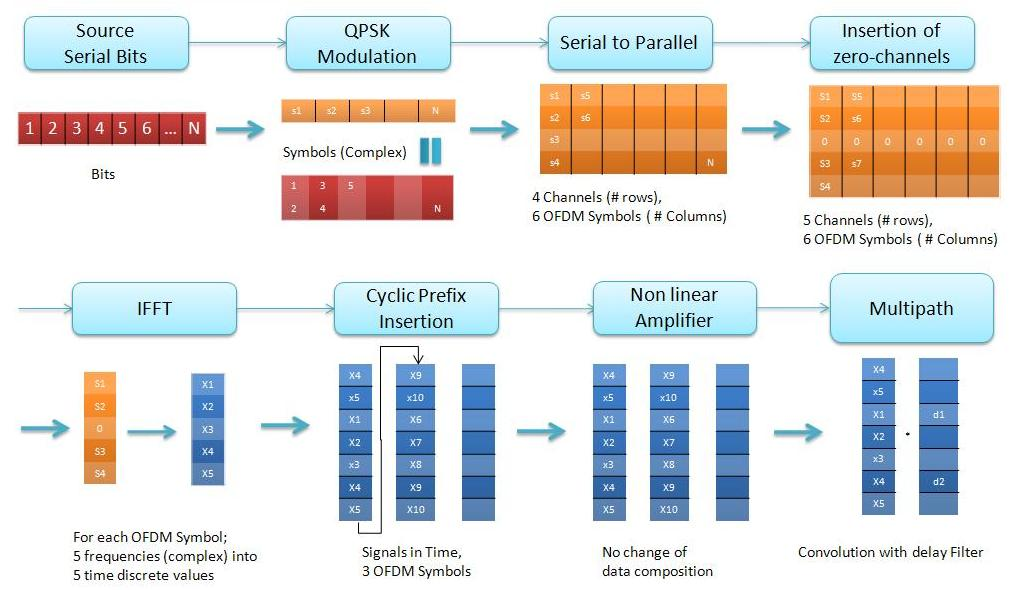
\includegraphics[width=\textwidth]{content/fig6/ofdmmodel1.JPG}
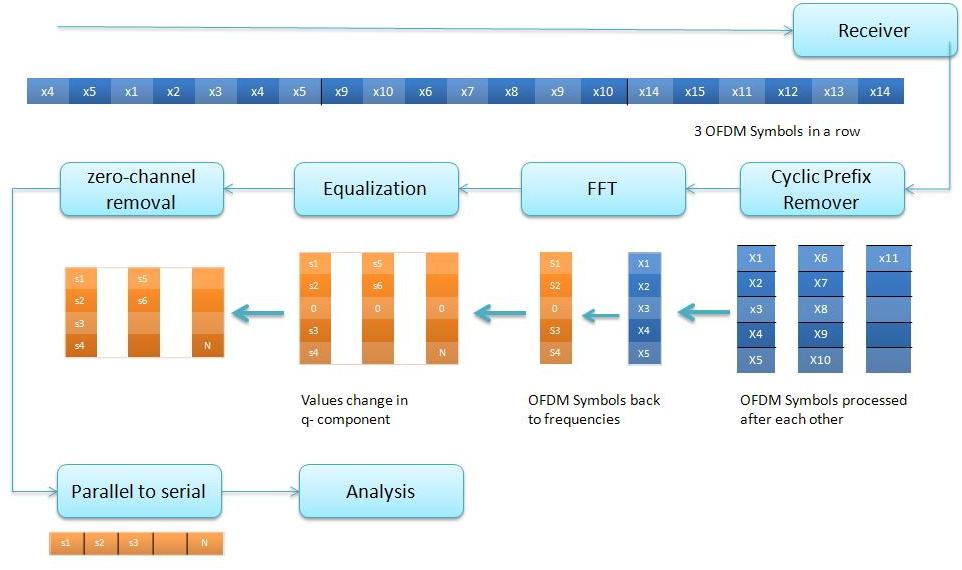
\includegraphics[width=\textwidth]{content/fig6/ofdmmodel2.JPG}
\caption{OFDM System Model}
\label{fig_ofdmsystemmodel}
\end{figure}

Figure \ref{fig_ofdmsystemmodel} presents the OFDM system block diagram.
Basic steps of the praxis are realized in blocks in the simulation. Additionally is shown how the composition of data changes in the single steps of the system.\\
The first block represents the data source. They are the bits which an application may send. In the simulation it is realized by a random bit generator. The following QPSK modulation block converts this bits into symbols, which are complex numbers. Each symbol carries several bits. The third block is the first one actually relevant for OFDM. The serial symbol stream is converted into a channel and OFDM symbol structure. In the simulation it is represented in a matrix shape where the rows are different channels and each column is an OFDM symbol. This means that each OFDM symbol, formed by $c$ (\#channels) serial symbols (complex numbers), is distributed over the $c$ channels.\\
In the next step zero channels are added in order to separate well subsequent OFDM symbols. For the simulation structure zero rows are added in the middle of the matrix. The following block interprets each symbol (complex number) of an OFDM symbol as a orthogonal frequency and converts each OFDM symbol per IFFT into a vector of time discrete values of the same length. As sixth step the cyclic prefix insertion is done. In order to maintain orthogonality of the frequencies but prevent ISI, an amount of \textit{guard values} are copied from the end of each OFDM symbol to its beginning. The number of rows in the simulation matrix grows by that by the number of \textit{guard values}.\\
The following block is the NLA which depends on the optimization parameter $\beta$ (back-off). At this point the transmitter side ends. In order to simulate the multipath a convolution is made on each OFDM symbol with the delay filter. Since the simulation is made on each OFDM symbol separated, this operation works with a memory in order simulate a serial transmission.\\
The receiver side is just the opposite of the transmitter. In the cyclic prefix remover the copied values are deleted and the simulation matrix size decreases. The next block performs the FFT on each OFDM symbol which reconstructs the as frequencies interpreted complex numbers.\\ The following equalization block tries to remove the effect of the multipath. For the simulation a multiplication with the inverted transfer function of the multipath is operated. By this, only the phase of the complex symbols changes.\\ Finally, the zero channels are removed and the matrix structure is reconverted to a series of symbols. The following analysis is done on the received symbols and consequently they are not demodulated into a bitstream.